\RequirePackage{amsthm} %https://tex.stackexchange.com/questions/687324/unknown-theoremstyle-warning-with-springer-nature-template
\documentclass[sn-mathphys-num,iicol]{sn-jnl}

%\usepackage{sn-jnl.sty}
\usepackage{graphicx}%
\usepackage{multirow}%
\usepackage{amsmath,amssymb,amsfonts}%
\usepackage{amsthm}%
\usepackage{physics}
\usepackage{siunitx}
\usepackage{mathrsfs}%
\usepackage[title]{appendix}%
\usepackage{xcolor}%
\usepackage{textcomp}%
\usepackage{manyfoot}%
\usepackage{booktabs}%
\usepackage{algorithm}%
\usepackage{algorithmicx}%
\usepackage{algpseudocode}%
\usepackage{listings}%
\usepackage{newtxmath}%
\usepackage[tiny]{titlesec}%

\theoremstyle{thmstyleone}
\newtheorem{theorem}{Theorem}
\newtheorem{proposition}[theorem]{Proposition}

\theoremstyle{thmstyletwo}
\newtheorem{remark}{Remark}

\theoremstyle{thmstylethree}
\newtheorem{definition}{Definition}

\raggedbottom

\newcommand{\td}{\text{d}}

\titleformat{\subsection}{}{\thesubsection}{1em}{\itshape}

\begin{document}
        
\title[Title]{Das Magnetische Moment des Protons}
\author*[1]{\fnm{Jonas} \sur{Wortmann}}\email{s02jwort@uni-bonn.de}
\affil*[1]{Rheinische Friedrich--Wilhelms--Universität, Bonn}

\abstract{Es wird das magnetische Moment des Protons in Bezug auf seine historische Bedeutung als erstes Indiz für die Substruktur des Protons erläutert.
Dafür wird der experimentelle Aufbau aus 1933 von \textsc{Frisch} und \textsc{Stern} zur Bestimmung des Protonenmoments erklärt, die Auswertung dargestellt und das Ergebnis in Hinblick auf die damaligen Erwartungen diskutiert.
Zu Beginn wird die Entdeckung des Protons durch \textsc{Rutherford} und das magnetische Moment und das Magneton dargestellt.
Im Anschluss wird ein Ausblick in aktuelle Forschungsthemen besprochen.}

\maketitle

\section{Einleitung}
Das Protonenmoment ist eine wichtige physikalische Größe, nicht nur im Kontext historischer Betrachtung, sondern auch vor dem Hintergrund der aktuellen Forschung.

Historisch führte das Protonenmoment zu Überlegungen über den Aufbau der Protonen.
Durch Messung des magnetischen Moments konnte erkannt werden, dass die damals gängige Theorie des Protons den experimentellen Ergebnissen nicht genügt.

In der aktuellen Forschung findet sich das Protonenmoment vor Allem im Vergleich mit dem Antiprotonenmoment, um Aussagen über die Charge--Parity--Time--Symmetrie (CTP--Symmetrie) und Materie--Antimaterie Asymmetrie zu treffen.
Ein großer Anwendungsbereich in der Medizin ist die Magnetresonanztomographie, die es ermöglicht, ohne schädliche Strahlung, Bilder von Gewebe zu erzeugen.

\section{Die Entdeckung des Protons}
Die Entdeckung des Protons wird im allgemeinen \textsc{Rutherford} um 1920 zugeschrieben.

In einem Experiment um 1913 beschossen \textsc{Rutherford} und \textsc{Mardsen} ein Gasgemisch (Luft) mit $\alpha $--Teilchen, um den inneren Aufbau der Atome zu erforschen.

Die $\alpha $--Teilchen stammen aus einer radioaktiven Probe, deren Teilchenstrahl auf Luft gerichtet ist.
Ein Zinksulfidschirm ist um die Luft herum angebracht, welcher als Teilchendetektor dient.
Die Entfernung des Schirms von dem Gas ist wesentlich größer als die Reichweite der $\alpha $--Strahlung, um zu vermeiden, das diese auf dem Schirm detektiert werden.

Das Ergebnis des Experiments zeigt, dass die $\alpha $--Teilchen mit der Luft stoßen und dabei Wasserstoffkerne aus dem Gas lösen, welche als Aufblitzen auf dem Schirm beobachtbar sind.

\textsc{Rutherford} wiederholte das Experiment mit Stickstoff.
Hierbei konnte er das selbe Aufblitzen wie bei Luft beobachten, woraus er schlussfolgerte, dass Stickstoff aus Wasserstoffkernen bestehen muss.

Die Entdeckung des Protons wird einer Aussage um 1920 von \textsc{Rutherford} zugeschrieben, bei der er seine Beobachtungen aus dem Experiment verallgemeinerte.
Er behauptete, dass jedes Atom aus Wasserstoffkernen bestehen musste.
Zur Unterscheidung von ionisiertem Wasserstoff, nannte er diese Bestandteile Protonen.\cite{Rutherford_proton_discovery}\cite{Rutherford1919}

\section{Das magnetische Moment und das Magneton}
Die klassische Betrachtung des magnetischen Moments des Protons liefert die Stärke und Richtung eines magnetischen Dipols $\boldsymbol{m}~=~\tfrac{1}{2}\int\td ^3r\left[\boldsymbol{r} \times \boldsymbol{j} \left(\boldsymbol{r} \right)\right]$.
Betrachtet man einen Strom der um eine Fläche kreist, so ergibt sich der Ausdruck $\boldsymbol{m} =I\cdot \boldsymbol{A} $.
Betrachtet man den Kreisstrom, erzeugt von einem geladenen Teilchen auf einer Kreisbahn, so ergibt sich mit $I=q/T$, mit der Periodendauer $T$ und der Ladung $q$, und der Kreisfläche $|\boldsymbol{A} |~=~\pi r^2$ ein Moment von $|\boldsymbol{m} |~=~\tfrac{q}{T}\pi r^2$.
Der Bahndrehimpuls eines Teilchens auf einer Kreisbahn wird beschrieben durch $|\boldsymbol{l} |=\tfrac{2\pi }{T}mr^2$.
Bahndrehimpuls und magnetisches Moment lassen sich also miteinander verbinden zu $|\boldsymbol{\mu } |~:=~|\boldsymbol{m} |~=~\gamma |\boldsymbol{l} |~=~\tfrac{q}{2m}|\boldsymbol{l} |$.
Diese Größe wird auch als Magneton bezeichnet.

Die quantenmechanische Betrachtung des Magnetons liefert dann diskrete Werte, die proportional zu den Eigenwerten von $\hat{l}_z$ sind.
Wichtig für die folgende Diskussion sind das \textsc{Bohr}'sche Magneton für Elektronen mit der Drehimpulsquantenzahl $\ell=1$: $\mu _B=\tfrac{e\hbar }{2m_e}$; und das Kernmagneton, eine gängige Einheit in der Teilchenphysik, für Teilchen mit Spin $\tfrac{1}{2}$, $\ell=1$ und der Protonmasse: $\mu _N=\tfrac{e\hbar }{2m_p}$.

\section{Das Experiment von Otto Robert \textsc{Frisch} und Otto \textsc{Stern}}
\subsection{Motivation}
Die Motivation hinter diesem Experiment ist die Untersuchung des Wasserstoffs mit dem Ziel der Bestimmung des Protonenmoments.
Darüber hinaus soll auch eine allgemeine Apparatur zur Messung magnetischer Momente in der Größenordnung eines Kernmagnetons $\mu _N$ errichtet werden.
Die kürzliche Entdeckung des Ortho-- und Para--Wasserstoffmoleküls sind hierfür nützlich und wollen auch untersucht werden.

\subsection{Experimenteller Aufbau}
\begin{figure}[h]
        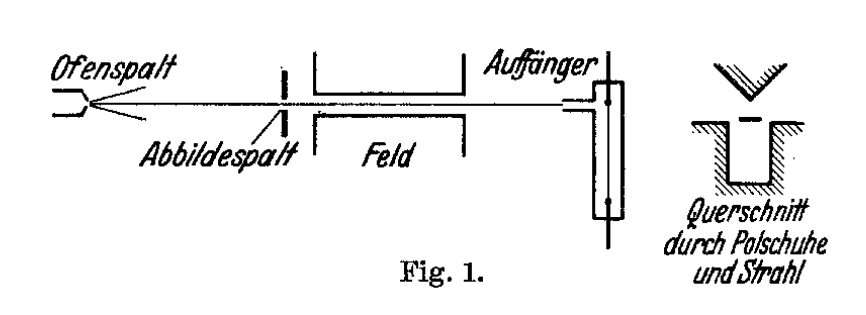
\includegraphics[width=.5\textwidth]{../vortrag/prosi_versuchsaufbau_mag_moment.png}
        \caption{Experimenteller Aufbau (schematisch); Gesamtlänge $\SI{30}{cm}$.\cite{FrischStern1933}}\label{fig:experimenteller_aufbau_frisch_stern}
\end{figure}
\noindent Der schematische experimentelle Aufbau ist in Abb.\ (\ref{fig:experimenteller_aufbau_frisch_stern}) gezeigt.
Aus dem Ofen tritt ein Molekülstrahl ($\text{H}_2$) aus, der mit Hilfe eines Abbildespaltes kollimiert wird und in ein inhomogenes Magnetfeld eintritt.
In diesem Feld wird der Strahl abgelenkt und die Intensität kann mit Hilfe des Auffängers (Manometer) gemessen werden.
Das Feld entsteht durch Polschuhe, deren Querschnitt abgebildet ist.
Auf die exakte Anordnung und technische Details wird hier nicht weiter eingegangen.
Diese sind ausführlich in der Originalarbeit\cite{FrischStern1933} erklärt.

Im Folgenden werden die Anforderungen und Schwierigkeiten aufgeführt.
Der Strahl muss aufgrund der kleinen magnetischen Momente äußert lang und schmal sein, damit die Abweichungen aufgrund der Feldeinwirkung entsprechend groß und genaue Messungen möglich sind.
Der kleinste im Experiment verwendete Strahl hat einen Durchmesser von circa $\SI{0.03}{mm}~=~\SI{30}{\micro m}$.
Wichtig sind große Inhomogenitäten im Feld.
Diese liegen im Bereich von circa $\SI{22}{T/cm}$.
Für einen Strahl mit einem magnetischen Moment von einem Kernmagneton ist dann eine Abweichung von $s~=~\SI{0.0044}{mm}~=~\SI{4.4}{\micro m}$ zu erwarten.

Besondere Schwierigkeiten ergeben sich aus der Natur des Molekülstrahls ($\text{H}_2$).
Die Moleküle im Strahl sind \textsc{Maxwell}--verteilt, was dazu führt, dass sie unterschiedliche Geschwindigkeiten haben und dadurch unterschiedlich starke Ablenkungen erfahren.
Aus diesem Grund kann die Ablenkung -- alleine verursacht durch das magnetische Moment -- nicht abgelesen werden, sondern muss aus der Intensitätsverteilung des Strahls berechnet werden.
Solch kleine Intensitäten können mit Hilfe sehr empfindlicher Manometer gemessen werden.
Technische Details sind in der Originalarbeit\cite{FrischStern1933} zu finden.

\subsection{Erwartungen}
Die Erwartung an das Experiment gibt für das Protonenmoment einen Wert von $\mu _p~=~1\cdot \mu _N~=~1\cdot \tfrac{e\hbar }{2m_p}$ an.
Diese Erwartung beruht auf der Annahme, dass das Proton ein elementares \textsc{Dirac}--Teilchen ist; also punktförmig und ohne innere Struktur.
Diese Annahme liegt in anbetracht des wissenschaftlichen Standes sehr nahe, da unter anderem das Elektron passend durch die \textsc{Dirac}'sche--Theorie beschrieben ist.

Der Wert des Protonenmoments sollte sich also, nur aufgrund des Massenunterschieds, um einen Faktor von circa 1840 von dem des Elektrons unterscheiden.\cite{FrischStern1933}

\subsection{Durchführung \& Auswertung}
Das Gesamtmoment des $\text{H}_2$ ist eine Zusammensetzung aus dem Rotationsmoment und dem Kernmoment.
Das Kernmoment ist nicht exakt das Protonenmoment, da es sich hier um das $\text{H}_2$--Molekül handelt; das Protonenmoment kann aber aus dem Kernmoment berechnet werden.

Die Beobachtung und Auswertung werden an Ortho-- und Parawasserstoffmolekülen durchgeführt, da ihre magnetischen Eigenschaften hilfreich zur Bestimmung der einzelnen Momente sind.

Das $\text{H}_2$--Molekül hat, aufgrund des \textsc{Pauli}--Prinzips, zwei mögliche Spinanordnungen.
In Ortho--$\text{H}_2$ ist die Ausrichtung $\ket{\uparrow\uparrow}$ zu finden; in Para--$\text{H}_2$ $\ket{\uparrow\downarrow}$.
Die Auswirkung davon ist, dass Ortho--$\text{H}_2$ ein Kernmoment ungleich null und Para--$\text{H}_2$ ein Kernmoment gleich null hat.
Für beide Arten des Moleküls erwartet man daher unterschiedliche Aufspaltungsbilder.
In Abb.\ (\ref{fig:ortho_aufspaltung}) ist dies beispielhaft für Ortho--$\text{H}_2$ gezeigt. 
\begin{figure}[h]
        \centering
        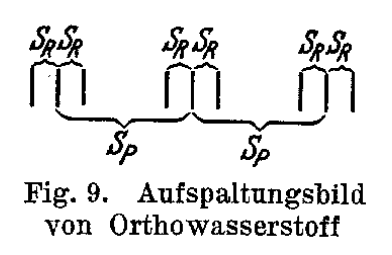
\includegraphics[width=.3\textwidth]{../vortrag/prosi_aufspaltungsbild_orthowasserstoff.png}
        \caption{Das Aufspaltungsbild von Ortho--$\text{H}_2$.\cite{FrischStern1933}} \label{fig:ortho_aufspaltung}
\end{figure}
Dabei beschreibt $S_R$ die Aufspaltung aufgrund des Rotationsmoments und $S_P$ die Aufspaltung aufgrund des Kernmoments.

Ziel dieser Auswertung ist die Bestimmung des Kernmoments, um Rückschlüsse auf das Protonenmoment zu ziehen.
Dafür muss das Rotationsmoment von $\text{H}_2$ bestimmt werden, um dieses im Anschluss von dem Gesamtmoment zu subtrahieren.
Die Berechnung folgt aus der Intensitätsverteilung von Para--$\text{H}_2$ (zu sehen für gewöhnliches $\text{H}_2$ in Abb.\ (\ref{fig:graph})), da eine Bestimmung durch direkte Auswertung der Ablenkung des Strahls aufgrund der Messgenauigkeit nicht möglich ist.
Para--$\text{H}_2$ wird deshalb verwendet, weil sein Kernmoment null ist und daher das Gesamtmoment nur aus dem Rotationsmoment besteht.
\begin{figure}[h]
        \centering
        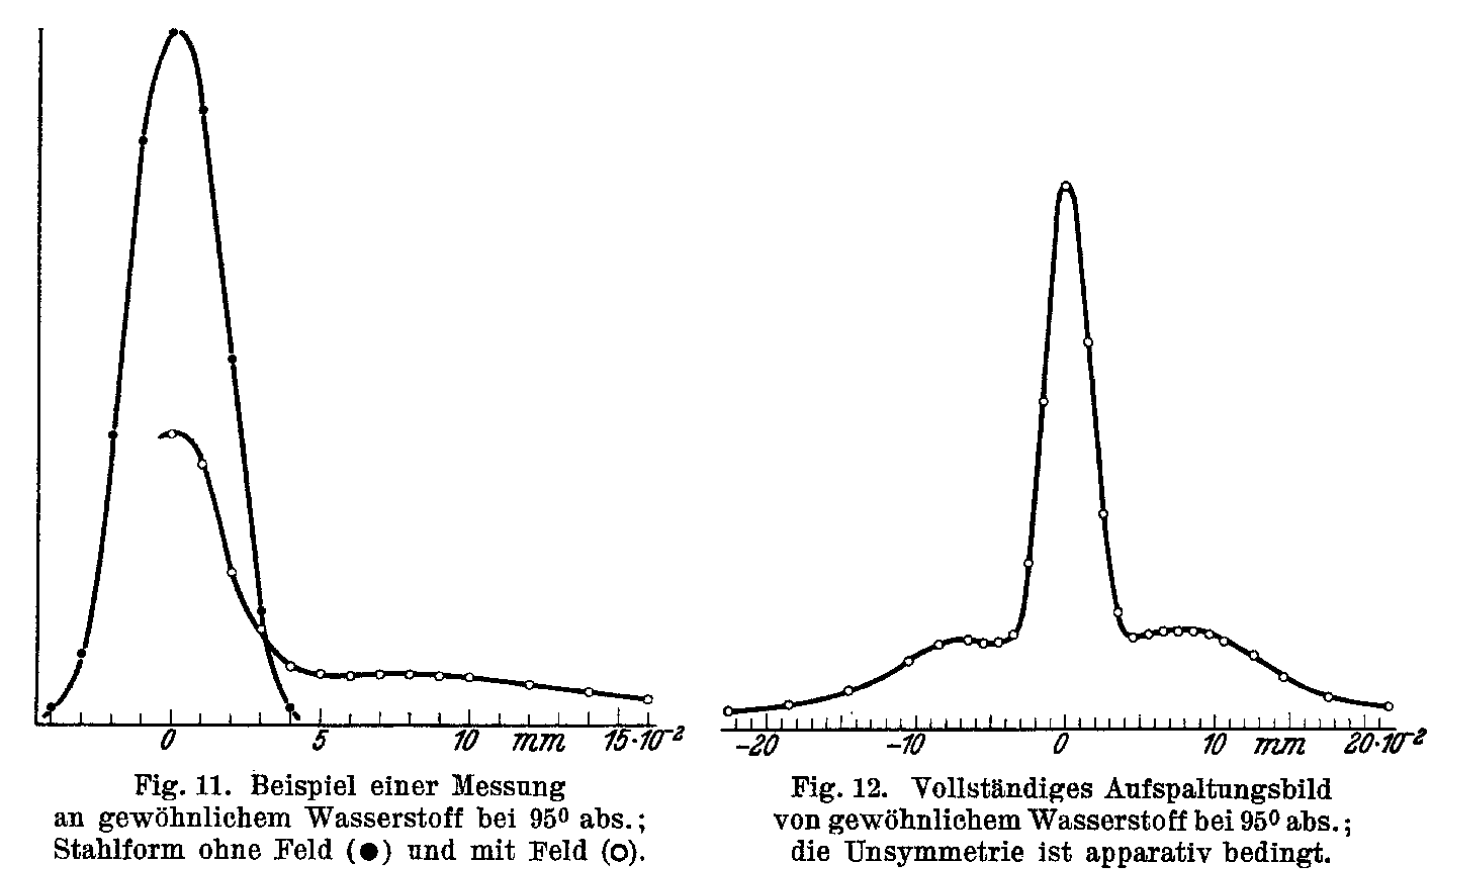
\includegraphics[width=.5\textwidth]{../vortrag/prosi_frisch_stern_auswertung_graph.png}
        \caption{Intensitätsverteilung des Molekülstrahls. Rechts ist eine Vergrößerung.\cite{FrischStern1933}} \label{fig:graph}
\end{figure}

Para--$\text{H}_2$ ist \textsc{Boltzmann}--verteilt, was bedeutet, dass $73\%$ der Moleküle die Rotationsquantenzahl $n=0$ und $27\%$ $n=2$ haben.
Für den Anteil mit $n=0$ ergibt sich keine Ablenkung, was dem Peak der Intensitätsverteilung um die Ablenkung von $\SI{0}{mm}$ entspricht (s.\ Abb.\ \ref{fig:graph}).
Für den Anteil mit $n=2$ ergibt sich eine Aufspaltung aufgrund der Aufhebung der Entartung.
Man erhält dann jeweils Anteile der Intensitäten von $\tfrac{1}{5}$ für $m_n\in\left\{-2,-1,0,+1,+2\right\}$ die je ein abiträres Rotationsmoment (--quant) von $m_n\cdot \mu _R$ besitzen.
Es ergibt sich also ein analoges Bild zu Abb.\ (\ref{fig:ortho_aufspaltung}) nur mit 5 anstatt 9 Intensitätsmaxima.

Dieses Rotationsmoment $\mu _R$ wird dann wie folgt bestimmt.
Man berechnet eine erwartete Intensität für ein gewähltes $\mu _R$ und vergleicht diese dann mit der tatsächlich gemessenen Intensität.
Stimmen diese Intensitäten nicht überein, so wird $\mu _R$ weiter variiert.
Für ein ausgezeichnetes $\mu _R$, was genau dem Rotationsmoment des Molekülstrahls entspricht, sind diese Intensitäten gleich.

Das Rotationsmoment von Para--$\text{H}_2$ ergibt sich dann zu $\mu _R\lesssim \mu _N$.
Dieses Rotationsmoment ist auch der Wert für gewöhnliches $\text{H}_2$.
Misst man also das Gesamtmoment über die selbe Methode so kann das Kernmoment von $\text{H}_2$ berechnet werden.\cite{FrischStern1933}

\subsection{Ergebnis}
Die im vorigen Abschnitt diskutierte Auswertung gibt für das magnetische Moment des Protons einen Wert von $3\mu _N\leq \mu _p\leq 5\mu _N$.
Dieses Ergebnis ist nicht mit der Erwartung von $\mu p~=~\mu _N$ vereinbar \cite{FrischStern1933}.
Aus moderner Forschungsperspektive ist dieser Wert hingegen sehr gut zu erklären.
Das Proton ist kein elementares Punktteilchen, sondern ein aus Quarks zusammengesetztes Teilchen $\left(u,u,d\right)$.
Das Protonenmoment berechnet sich also aus dem Moment der Quarks mit $\mu _p~=~\tfrac{3}{4}\mu _u~-~\tfrac{1}{3}\mu _d~\approx~ 2.792\mu _N$\cite{CODATA_proton_magneton}.

Obwohl dieses Ergebnis in der Originalarbeit noch nicht gedeutet werden konnte, ist es ein wichtiges Ereignis, bei dem die Struktur des Protons erstmals in Frage gestellt wurde.

\section{Die Substruktur des Protons}
Eine genaue Betrachtung der Substruktur von Teilchen haben zum ersten Mal \textsc{Gell--Mann}\cite{Gellmann1964} und \textsc{Zweig}\cite{Zweig1964} 1964 unabhängig voneinander angestellt.

\textsc{Gell--Mann}\cite{Gellmann1964} stellt ein Modell dar, indem Teilchen aus anderen Teilchen, namentlich \textit{Quarks}, aufgebaut werden können.
Es ergibt sich, dass Baryonen aus einer ungeraden Anzahl an Quarks, also $\left(q,q,q\right)$, $\left(q,q,q,q,\overline{q}\right)$ etc.\ und Mesonen aus einer geraden Anzahl, also $\left(q,\overline{q}\right)$, $\left(q,q,\overline{q},\overline{q}\right)$ etc.\ aufgebaut werden können.
Er zeigt, dass der von ihm beschriebene \textit{Eightfold Way} zur Kategorisierung von Teilchen mit seinem Quark--Modell vereinbar ist.

Eine analoge, allerdings nicht auf dem \textit{Eightfold Way} beruhende Erklärung wird auch von \textsc{Zweig}\cite{Zweig1964} geliefert.
In seiner Ausarbeitung stellt er diese Elementarteilchen als Aces vor.

Diese Modelle wurden kurz nach Veröffentlichung beider Arbeiten am SLAC (Stanford Linear Accelerator Center) Experiment bestätigt.\cite{Bloom1969}
Bei Elektron -- Proton Streuung wurde der Formfaktor gemessen, welcher ergab, dass die Ladungsverteilung innerhalb des Protons punktförmig sein musste.
Dieses Ergebnis wurde in einer Ausarbeitung von \textsc{Bloom}, et al.\ \cite{Bloom1969} diskutiert und diese punktförmige Ladungsverteilung wurde mit den Quarks von \textsc{Gell--Mann} identifiziert.

\section{Aktuelle Forschung}
In der modernen Forschung findet das Protonenmoment eine große Bedeutung, vor Allem im Hinblick auf die CPT--Symmetrie und Materie--Antimaterie Asymmetrie.
Anwendung findet das Protonenmoment in der Medizin, genauer in der Magnetresonanzspektroskopie.

Am BASE im Cern\cite{BASE2017} wird mit Hilfe von zwei \textsc{Penning}--Fallen das magnetische Moment des Antiprotons gemessen und mit dem magnetischen Moment des Protons verglichen.
Dabei können die Zyklotronfrequenz und \textsc{Lamor}präzession jeweils separat gemessen werden, um eine möglichst hohe Auflösung zu erreichen.
Es wird nach Diskrepanzen gesucht, die zu möglichen Symmetriebrechungen führen könnten.
Bisher sind die Momente beider Teilchen innerhalb der Fehlergrenzen identisch.

Das MRT beruht auf der Spin--Gitter und Spin--Spin Relaxation der Protonen in einem (organischen) Material.
Die Spins werden mit Hilfe eines homogenen Magnetfeldes ausgerichtet und anschließend durch Impulse magnetischer Wechselfelder ausgelenkt.
Diese Auslenkung ruft zwei Effekte hervor:
Die Spin--Gitter Relaxation, bei der sich die Protonenspins langsam entlang der homogenen Magnetfeldlinien ausrichten und dabei eine Änderung der Magnetisierung in der zum Feld orthogonalen Ebene gemessen werden kann;
und, die Spin--Spin Relaxation, bei der eine abnehmende Magnetisierung innerhalb der orthogonalen Ebene gemessen werden kann, die aufgrund der unterschiedlichen Präzessionsgeschwindigkeiten der Protonenspins zustande kommt.
Bei beiden Relaxationsprozessen wird eine Magnetisierung gemessen, die computergestützt in Bilder von Spindichten umgewandelt werden kann.
Diese geben Aufschlüsse über die Beschaffenheit der untersuchten Probe.

\bibliography{refs}

\end{document}
